\chapter{Introduction and research statement}
A \textit{software process} is a set of activities leading to the design and development of software systems. Examples of such activities are design methods: such as requirements collection and creation of an UML diagrams; or testing strategies: such as requirements testing or performance analysis. The intent behind the software process is to structure and coordinate human activities in order to achieve the goal - deliver the software system. 

Many work has been done in the software process domain resulted in a number of industrial standard process models: CMM, ISO, PSP etc. \cite{citeulike:5043104}. Nevertheless, software development process stays error-prone and more than a half of all software development projects ending up failing or very poorly executed for many reasons. Some of them getting abandoned running out of budget, some delivered with so low quality or so late that they become useless and some, when delivered, never get used by prospective users because they do not fulfill original requirements. The cost of this lost effort is enormous and it clearly reveals our incomplete knowledge of the software process.

There is a long history of software process improvement through proposing specific patterns of software development process. For example, the Waterfall Model process proposes a sequential pattern in which developers first create a Requirements document, then create a Design, then create an Implementation, and finally develop Tests. The Test Driven Development process proposes an iterative pattern in which the developer must first write a test case, then write the code to implement that test case, then refactor the system for maximum clarity and minimal code duplication. One problem with the traditional top-down approach to process development is that it requires the developer or manager to notice a recurrent pattern of behavior in the first place \cite{citeulike:5043104}. 

\begin{figure}[tbp]
   \centering
   \includegraphics[height=65mm]{system_overview.eps}
   \caption{The high-level system overview. Software engineering process and product data collected and aggregated by Hackystat used to generate temporal symbolic indexes. Data mining tools constrained by the software engineering domain knowledge are then used for unsupervised patterns discovery. The GUI provides an expert interface for discovered patterns and knowledge base aiding iterative investigation of a discovered phenomena.}
   \label{fig:system_overview}
\end{figure}

In my research, I will apply knowledge discovery and data mining techniques to the domain of software engineering in order to evaluate their ability to automatically notice interesting recurrent patterns of behavior. I am not envisioning to be able to infer full complete and correct software process models but rather will develop a system which will provide a user with some formal description of discovered recurrent behaviors in the software process. As a simple example, consider a development team in which committing code to a repository triggers a build of the system. Sometimes the build passes, and sometimes the build fails. To improve the productivity of the team, it would be useful to be aware of any recurrent behaviors of the developers. My system might generate one recurrent pattern consisting of a) implementing code b) running unit tests, c) committing code and d) a passed build: $i \rightarrow u \rightarrow c \rightarrow s $, and another recurrent pattern consisting of a) implementing code, b) committing code, and c) a failed build: $i \rightarrow c \rightarrow f $. The automated generation of these recurrent patterns can provide actionable knowledge to developers; in this case, the insight that running test cases prior to committing code reduces the frequency of build failures.

Although, latest trends in the software process study emphasize mining of the software process artifacts and behaviours \cite{citeulike:5043664} \cite{citeulike:1885717} \cite{citeulike:5112229} \cite{citeulike:1885717}, to the best of my knowledge, the approach I am taking through the mining of 
automatically collected, low-level product and process data has never been attempted. The proposed contributions of my research will include: a) the implementation of a system aiding in discovery of novel software process knowledge (shown at the Figure \ref{fig:system_overview}); b) my experimental evaluation of the system which will provide insight into its strengths and weaknesses, and c) the possible discovery of useful new software process patterns.
